% IOE Graduate Conference Version 19.0 format.
% The class file is copied unchanged from the supplied IOEGC template.
\documentclass[fleqn,10pt,twoside]{IOEGC}

% Identified editorial version for submission to the 19th IOE Graduate Conference.

\PaperTitle{Graph-Attention Double-DQN for Cellular Handover: A Paired Simulation Evaluation}

\Authors{Saange Tamang\textsuperscript{a}, Sulav Kandel\textsuperscript{b}}

\Abstract{
Cell handover helps a moving phone stay connected as it moves between cells. A controller must decide when to switch. Switching too often can interrupt service, while staying on a weak cell can reduce data delivery. This study tests a graph-attention dueling Double DQN (DDQN) that selects the serving cell using simulated signal, load, and movement information. We compare three trained, fixed policies with a configured A3-style controller on 639 reserved route cases and 540 Pokhara transfer groups with simulated cell layouts. On the reserved routes, the learned policies have 8.9--10.0\% higher aggregate throughput and 36.1--53.0\% fewer handovers per hour. They also have fewer ping-pongs and less weak-service time, but a higher share of completed stays shorter than 5 s. In the Pokhara tests, throughput is 3.7--3.9\% higher, with fewer handovers, ping-pongs, and less weak-service time. Short-stay results differ by policy. We also tested a load-aware rule after reviewing the main results; it did not meet the development criteria. The tests use three training seeds, roads that partly overlap with training routes, simulated cell layouts, and information available only in the simulator. The results do not show field performance or prove that graph attention caused the differences.
}

\Keywords{cellular handover, graph attention, Double DQN, reinforcement learning, simulation}

\Affiliation{\textsuperscript{a,b} Paschimanchal Campus, Institute of Engineering, Tribhuvan University, Pokhara, Nepal}

\Email{\textsuperscript{a} connectwithsaange@gmail.com; \textsuperscript{b} connectwithsulav@gmail.com}

\hypersetup{pdfauthor={Saange Tamang, Sulav Kandel},pdftitle={Graph-Attention Double-DQN for Cellular Handover: A Paired Simulation Evaluation},pdfsubject={Submission to the 19th IOE Graduate Conference, 2026}}
\Archive{Submission to the 19th IOE Graduate Conference, 2026}

\begin{document}
\hypersetup{pdfsubject={Submission to the 19th IOE Graduate Conference, 2026}}
\maketitle
\thispagestyle{firstpage}

\section{Introduction}
When people move, their phones may move between cells. Signal strength and cell load can change along the way. If a phone stays with a weak cell for too long, service may suffer. If it switches whenever another cell looks slightly better, it may make too many handovers. A handover controller needs to balance service and switching.

LTE includes Event A3, which compares the signal from a neighbouring cell with the signal from the current cell. Hysteresis and a time-to-trigger help control when a handover starts \cite{3gpp36}. A learning controller that selects a serving cell makes a different decision from the full LTE handover procedure. In this study, we test that choice in a simulator. We do not model all of the signalling and network steps used in a live LTE system.

A handover does not always improve service. The new cell may have a weaker signal or more traffic. At the same time, staying connected to a weak cell can also reduce service. For this reason, we measure throughput, time with a weak signal, handovers, ping-pongs, and short cell stays. Handover count alone does not show whether users received better service.

We test a controller that uses graph attention and reinforcement learning. It treats cells as nodes and uses information from nearby cells. A dueling Double DQN then chooses the serving cell using simulated signal, load, and movement information. The radio and traffic conditions are generated by the simulator, so the results apply to the conditions used in these tests.

We compare three trained, fixed policies with a configured A3-style controller. The main tests include 639 reserved route cases and 540 transfer cases based on Pokhara roads and simulated cell layouts. We report throughput, handovers, ping-pongs, weak-service time, and short stays. We also report a load-aware diagnostic that was designed after we had seen the main results. Many roads in the reserved set also appear in training. The Pokhara tests use real road shapes but simulated cell layouts. These results are from simulation. They do not show how the controller would work in a live network, or whether graph attention itself caused the results.

\section{Literature Review}
LTE Event A3 provides a common reference for handover studies. It compares measurements from the serving cell and a neighbouring cell, with hysteresis and a time-to-trigger condition \cite{3gpp36}. Yue et al. adjusted the A3 margin and time-to-trigger using a handover-risk cue in a low-mobility simulation \cite{yue2026}. Our study looks at a different task: choosing a serving cell while a user travels on a road. The settings of an A3-style reference need to be stated because they affect the comparison.

Some studies use reinforcement learning to control handovers. Jang et al. used proximal policy optimisation for UAV handover and combined signal strength with a handover penalty \cite{jang2022}. Their results show that the penalty weight affects the balance between connection quality and switching. They use received signal strength as the service measure. In our road-mobility simulation, we also measure delivered data while background traffic is present.

Alizadeh, Lim, and Vu used multi-agent Q-learning for load balancing and user association \cite{alizadeh2024}. Their handover cost becomes smaller when a user has stayed with a cell longer. Our reward uses a fixed cost for each handover instead. We report short cell stays as a separate result.

Graph models have been used to share information between nearby cells. Mehrabi et al. used graph-convolutional models to represent nearby cells and changing traffic, then adjusted LTE A2 thresholds using two metro datasets \cite{mehrabi2023}. Yu et al. combined message-passing networks with deep Q-learning for satellite handover \cite{yu2024}. Those studies adjust thresholds or focus on satellite links. Our controller chooses a serving cell for road travel.

Other work has studied handovers for vehicles. Mehregan and De Grande proposed TH-GCN and measured throughput, SINR, packet delivery, handovers, and ping-pongs \cite{mehregan2025}. This shows why service and switching should be reported together. González Bermúdez et al. studied GNN-based prediction of user--cell links for O-RAN using real and emulated data \cite{gonzalez2025}. Link prediction may help prepare for handovers, but it does not by itself show what happens after a switch. Prediction and a controller that acts in a simulator answer different questions.

Salvatori et al. proposed dual-graph multi-agent reinforcement learning to adjust cell-individual offsets \cite{salvatori2026}. Their preprint tests network-level actions in ns-3, including changes in topology and transfer to an unseen Manchester area. Our study instead chooses a serving cell for one moving user. A model accepting a new graph does not by itself prove that it will provide good service on that graph. Also, using different route IDs does not mean that the roads are different if road segments overlap.

We evaluate three fixed policies selected using development routes. Each uses a handover cost of 0.875. We compare them with the same configured A3-style controller on reserved routes and on Pokhara roads with simulated cell layouts. We report throughput, handovers, ping-pongs, weak-service time, and short stays. The results describe this simulator only. They do not prove field performance or show that graph attention caused the observed differences.

\section{Theoretical Formulation and Methodology}
This chapter explains how the study was set up and how the controller was trained. The controller chooses which cell serves a moving user equipment (UE). It aims to provide good service while avoiding unnecessary handovers. The method uses information about nearby cells and a dueling Double-DQN. The sections below describe the routes, simulator, controller inputs, and training steps.

\subsection{Dataset construction and experimental partitions}
For the Kathmandu-area tests, we used road routes from OpenStreetMap \cite{osm} and a supplied layout with 46 sites. The simulator treats each site as one cell. We did not verify that the supplied coordinates match real operator sites. Routes stay fixed during a run; the simulator generates the signal, background traffic, resource use, and handover outcomes. Figure~\ref{fig:protocol} summarizes the route splits and the Pokhara transfer tests.

The route bank has 6,543 routes, grouped by origin and destination (OD). With a fixed random seed, we assigned 5,242 routes to training, 662 to development, and 639 to the reserved test set. These sets contain 812, 101, and 102 OD groups, respectively. We used six fixed routes for development checks. Routes with the same OD pair stayed in the same set. Different OD pairs may still share roads.

Some roads occur in more than one split. Of the directed road edges in the development set, 99.41\% also occur in the full candidate training set. For the reserved test set, the overlap with that candidate training set is 99.01\%. Each final training run used a fixed plan of 300 journeys, not all 5,242 training routes. Of the 49,679 distinct directed edges in the reserved test set, 33,340 (67.11\%) also occur in those 300 journeys. Each edge counts once in these percentages, regardless of its length or how often it is used. The reserved routes were not used for training, but many of their roads were. This is not a test on fully unseen roads.

The Pokhara transfer test uses 60 routes on real roads and three simulated cell layouts. Each layout has 46 cells and a different generation seed: 8101, 8102, or 8103. The routes are split into three length groups: 20 from 1 km to under 3 km, 20 from 3 km to under 6 km, and 20 from 6 km to under 12 km. We tested each route with all three layouts and three radio/traffic condition pairs. This gives 540 route--layout--condition groups and 2,160 runs across the A3-style controller and three trained policies. Since the same routes appear in several groups, the groups do not represent 540 different places. We did not use Pokhara results to tune the reward or select a training seed. All 540 planned groups are reported.
\begin{figure}[H]\centering
  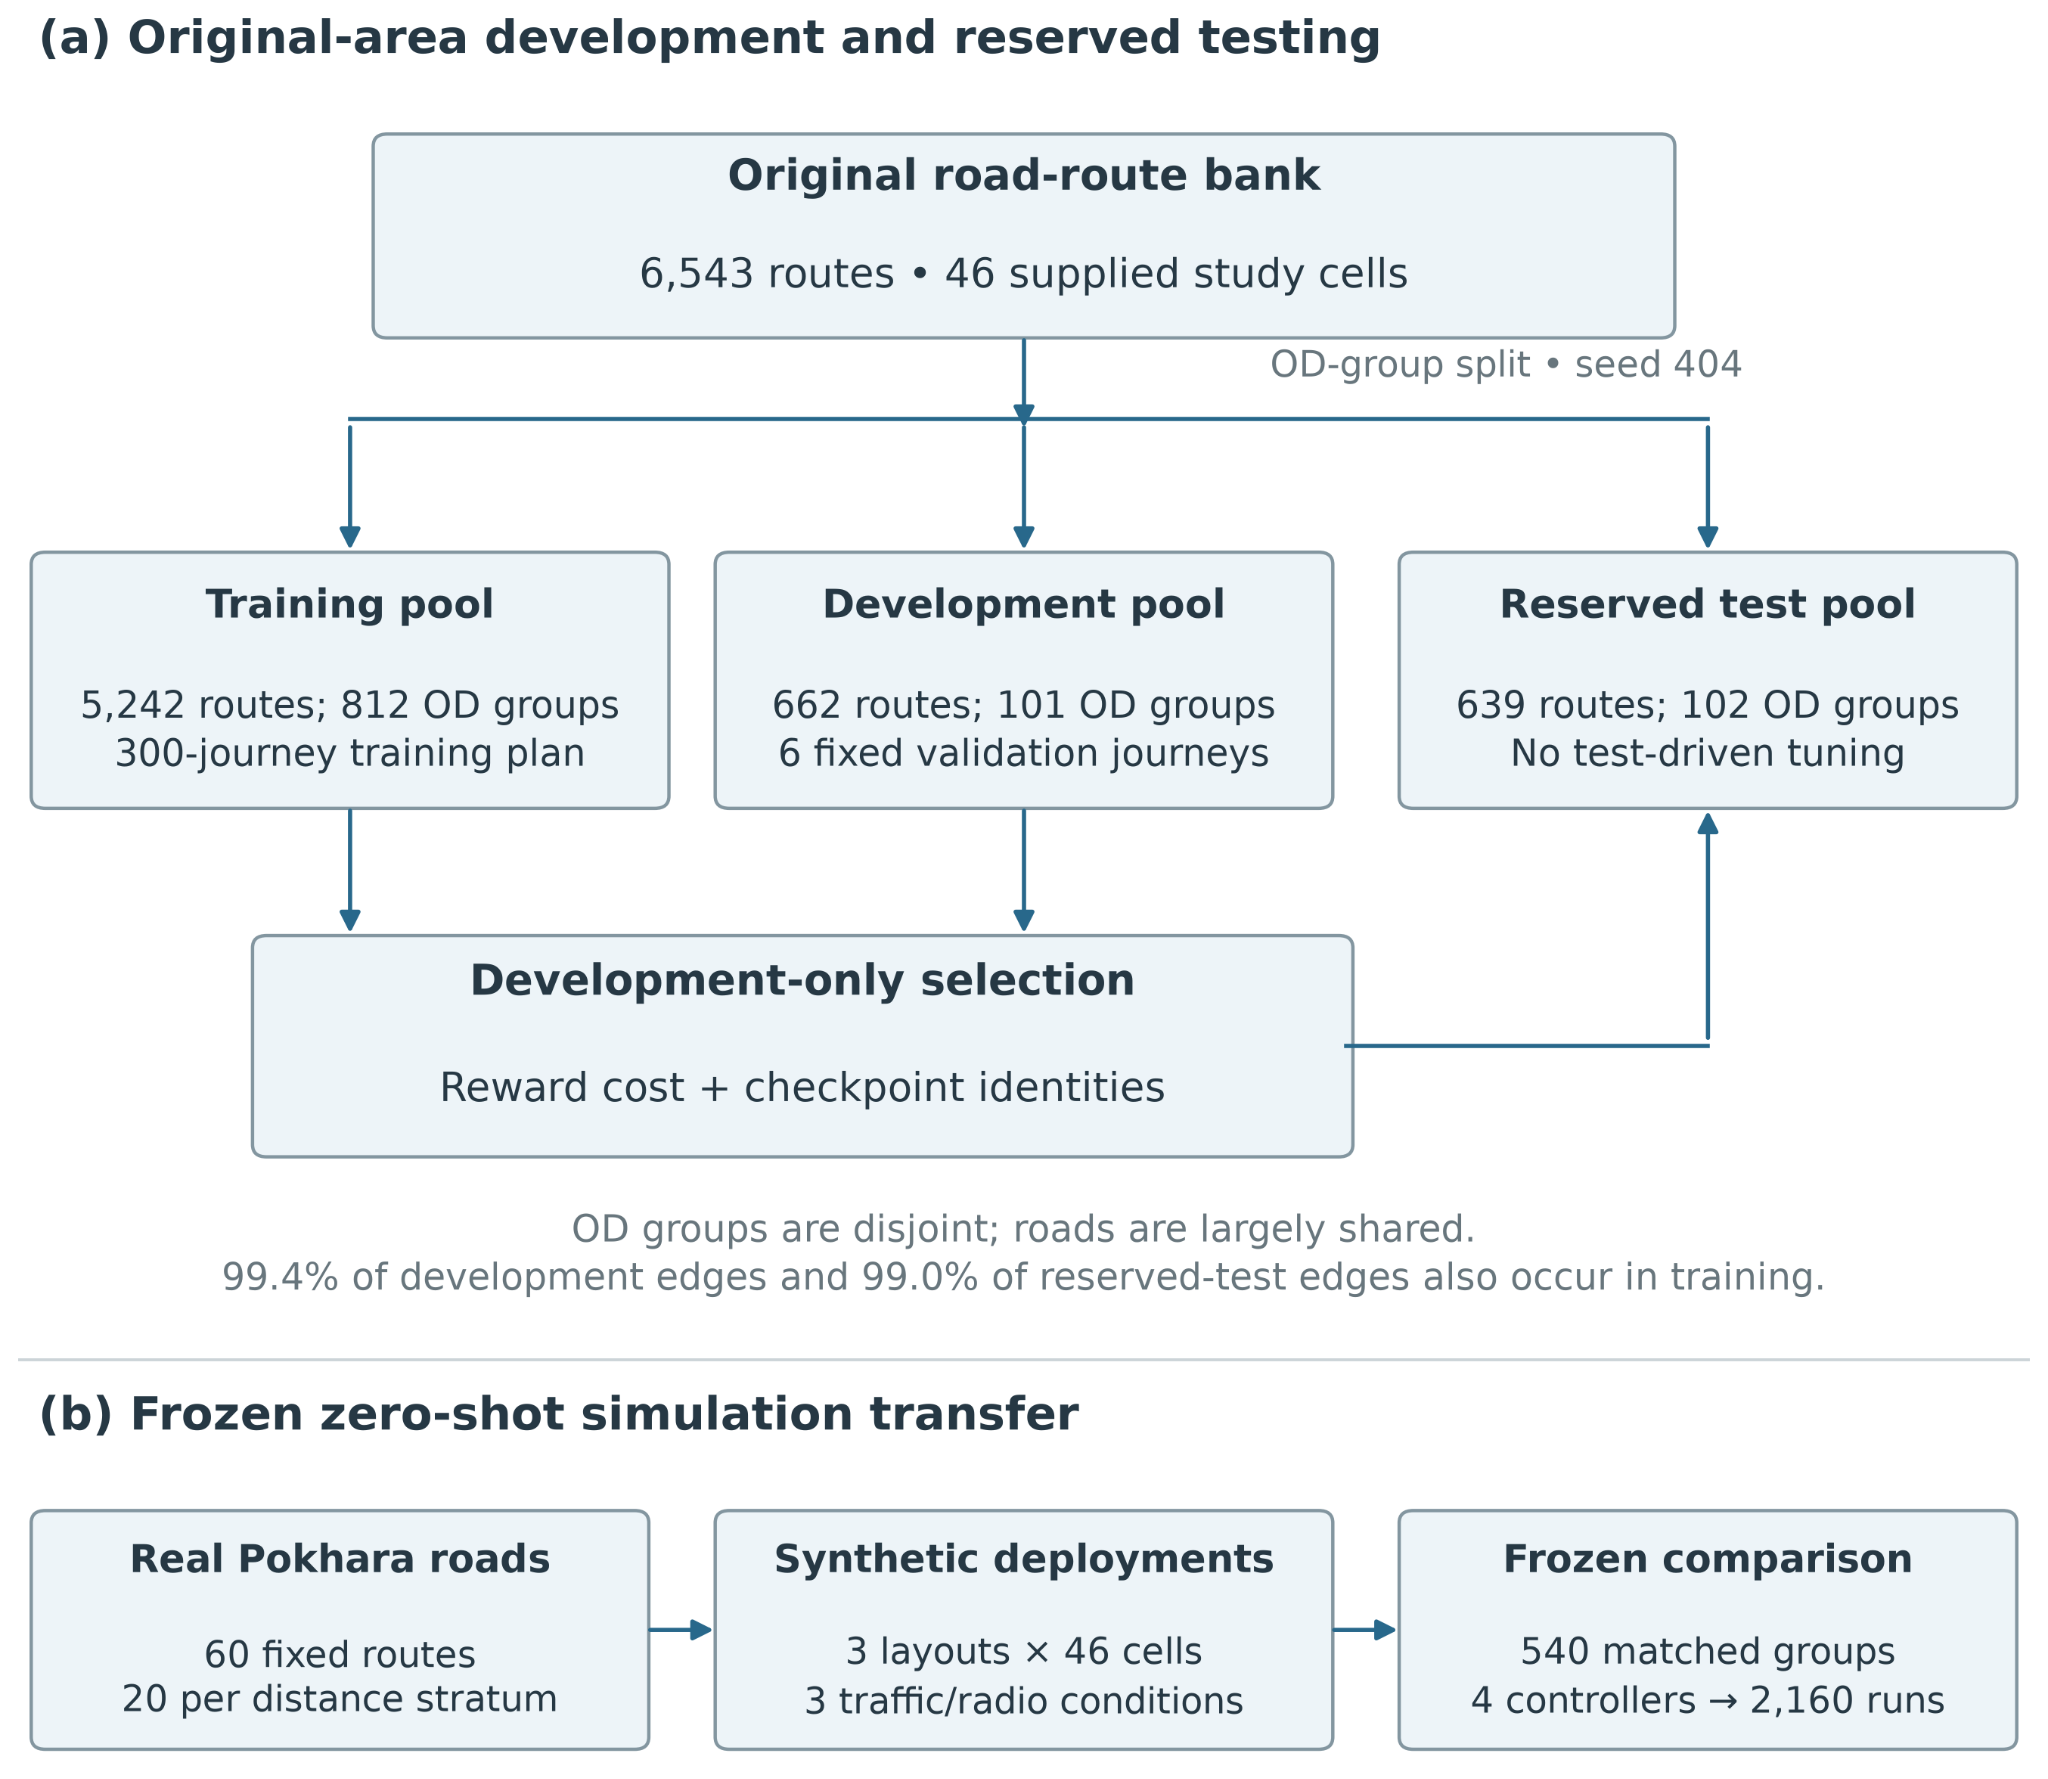
\includegraphics[width=0.98\linewidth]{Graphics/data-partition-and-transfer-protocol.png}
  \caption{Route partitions and transfer design. The 99.41\% and 99.01\% overlap figures use the full candidate training pool; overlap against the 300 executed journeys is 67.11\% of unique reserved-set edges. Pokhara uses real road geometry and synthetic cell layouts; all 540 planned groups are present.}
  \label{fig:protocol}
\end{figure}

\subsection{Network, mobility, and modelling assumptions}
We model the cells as a graph $G_c=(V,E_c)$. Each of its $N=46$ nodes represents one supplied cell location $b_i$. Two different cells are linked if they are at most 1,500 m apart; the original layout has 96 such links. Links work in both directions. Each node also has a self-loop, so the model can use that cell's own information. A self-loop does not allow a handover back to the same cell. This graph describes cell proximity; it is separate from the road map and does not represent backhaul links or a confirmed operator neighbour list. Figure~\ref{fig:layout} shows the cell locations and proximity links. The map source and attribution are given in the figure and reference list \cite{osm}.

Each episode follows one road journey at 10 m/s. The controller makes a decision every 0.5 s, except that the last interval is shortened if less than 0.5 s remains. At the start, the UE connects to the cell with the strongest modelled reference signal received power (RSRP). A switch to another cell causes a 0.1 s service interruption. If it continues into the next interval, the remaining interruption time is carried forward. No further handover is allowed until it ends. The controller can change the serving cell, but not the route, speed, or transmission settings. The model assumes flat ground and does not include fast fading or sector antenna patterns.

\begin{figure}[H]\centering
  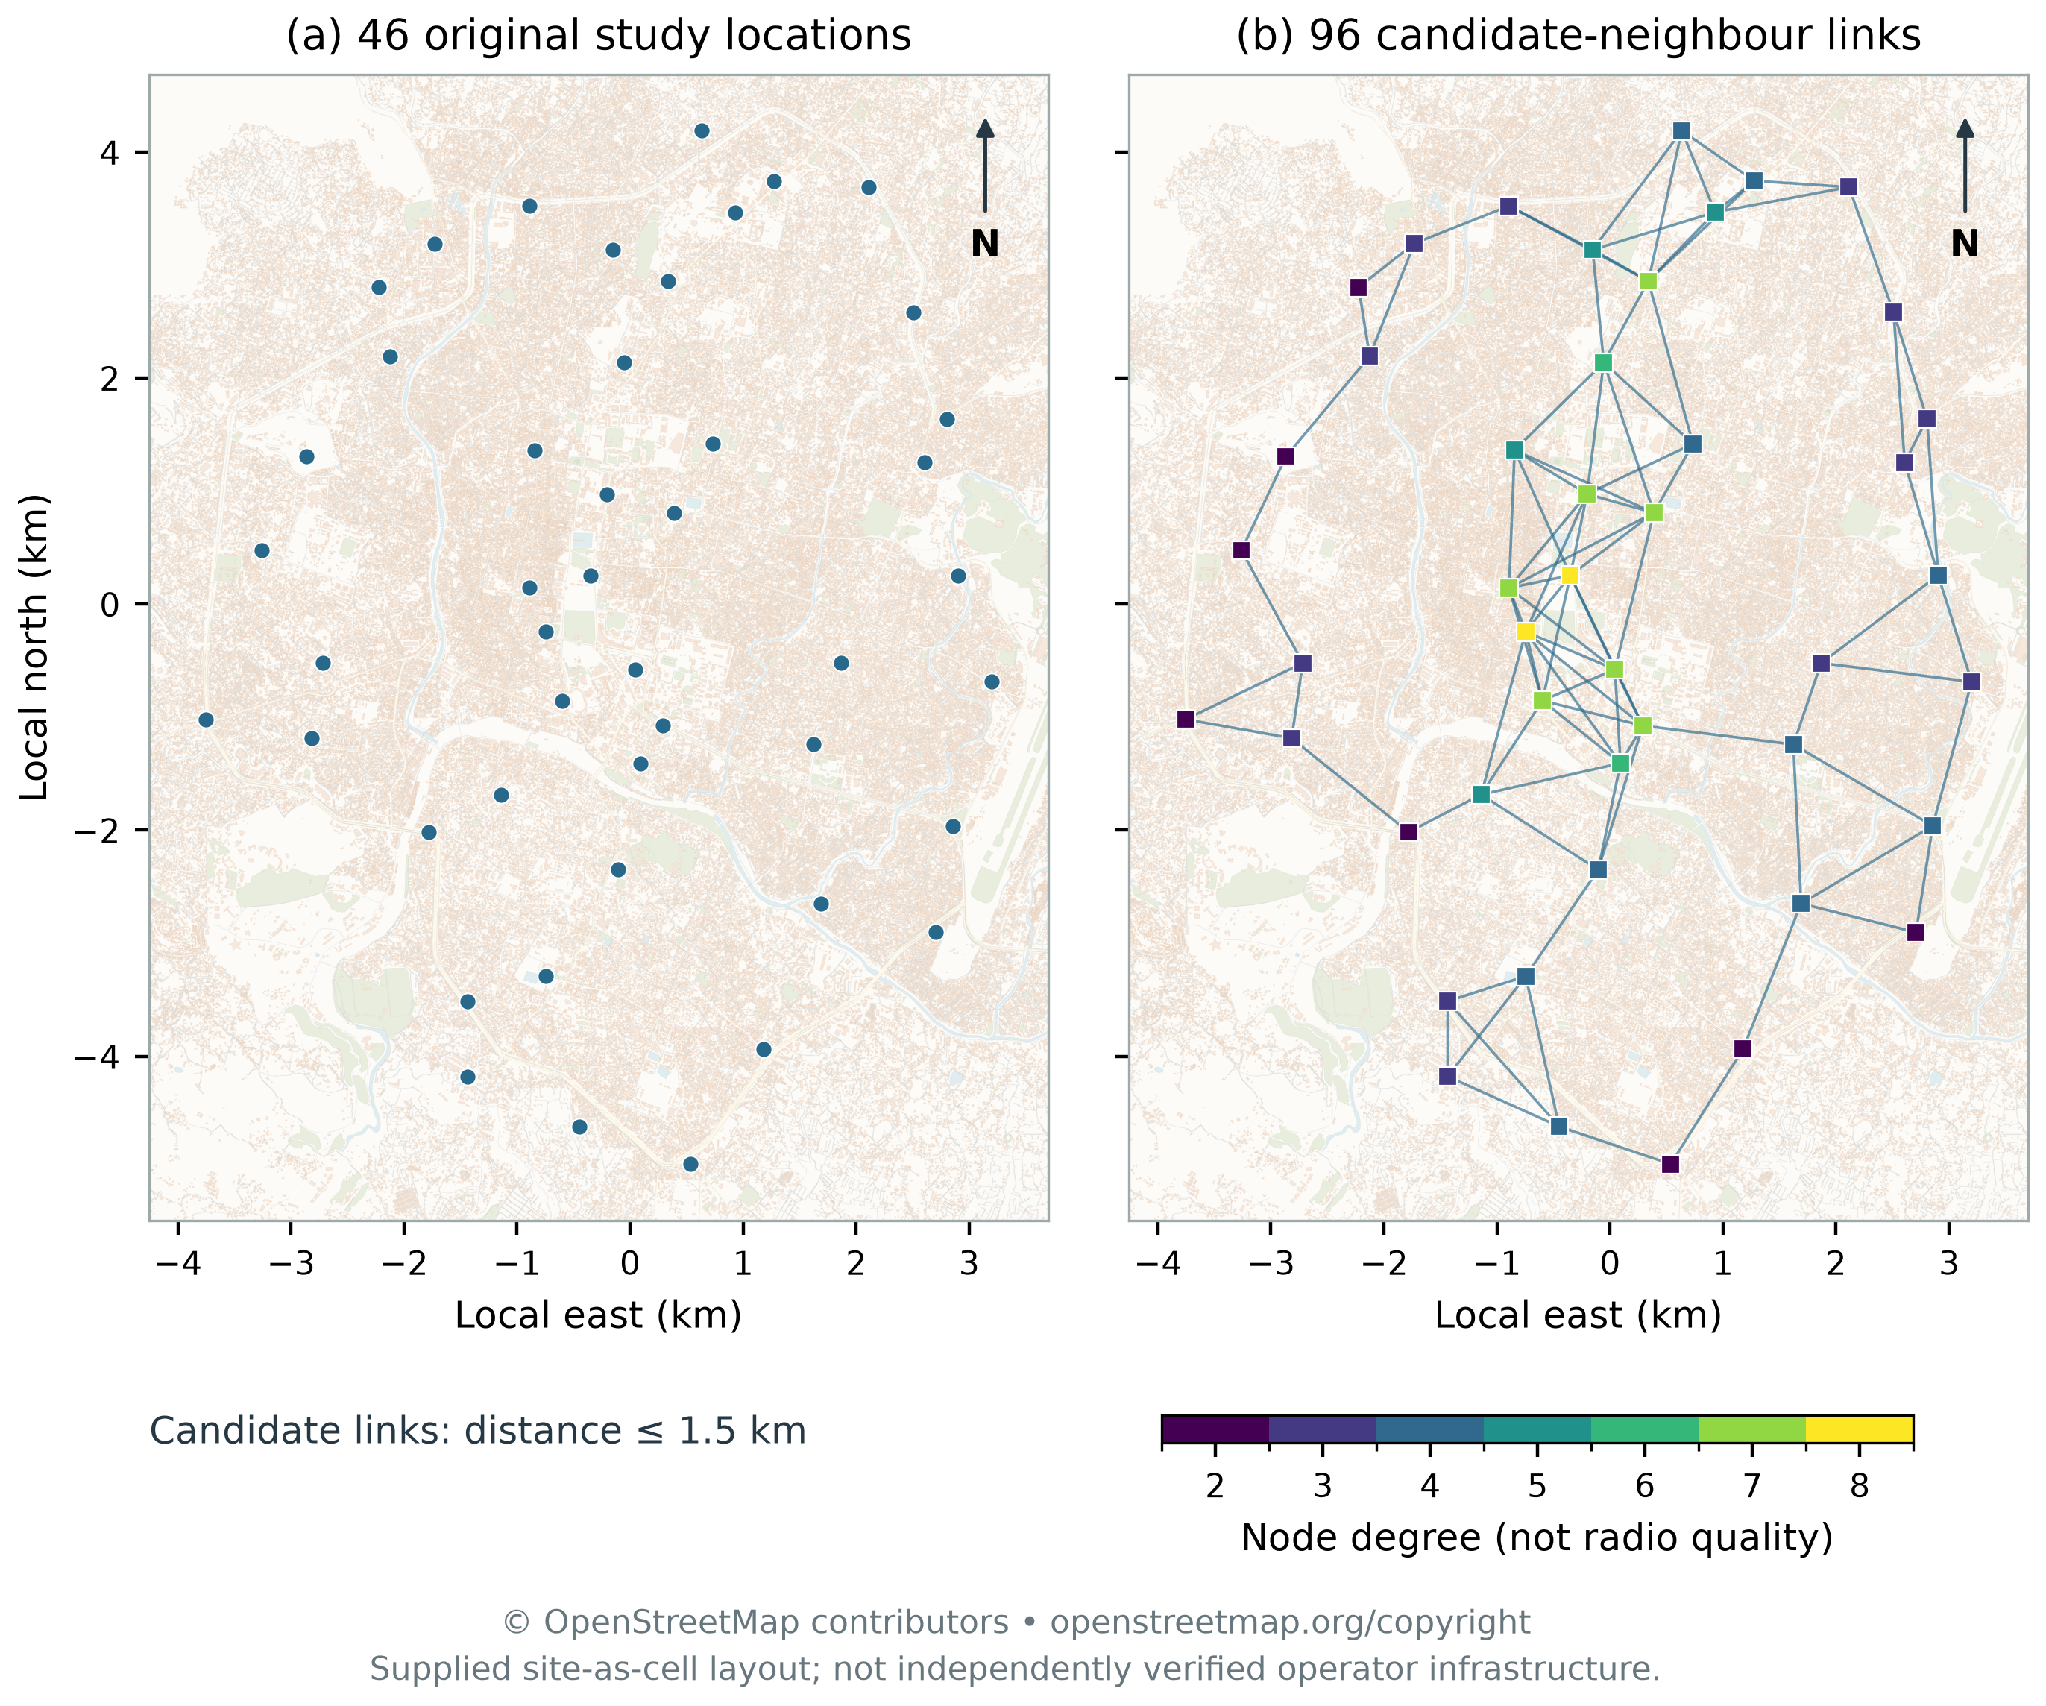
\includegraphics[width=0.98\linewidth]{Graphics/cell-layout-and-neighbor-graph.png}
  \caption{Cell locations supplied for this study and the proximity links used in the cell graph. A link joins two cells no more than 1.5 km apart. Node colour shows the number of neighbouring cells, not signal quality. The locations were not verified as operator sites. Map data \copyright{} OpenStreetMap contributors (ODbL); attribution and license: \url{https://www.openstreetmap.org/copyright}.}
  \label{fig:layout}
\end{figure}

\subsection{Radio model, background traffic, and delivered service}
We estimate signal power with an urban macrocell path-loss model adapted from 3GPP TR~36.942 \cite{3gpp942}. It includes a free-space-based minimum path loss and spatially correlated log-normal shadowing. Shadowing has a 4 dB standard deviation and a 20 m correlation distance. Signal and noise are calculated for each subcarrier.

For each cell $i$ and time $t$, the simulator calculates the signal-to-interference-plus-noise ratio (SINR), $\xi_{i,t}$. It then estimates the UE's rate, $C_{i,t}^u$, if that cell used all of its radio resources. The rate is in Mbps:
\begin{equation}
  \begin{aligned}
  \xi_{i,t}&=\frac{S_{i,t}}{N_0+\sum_{j\ne i}\alpha_{j,t}\omega_{ij}S_{j,t}},\\
  C_{i,t}^u&=\eta B_i\min\{\log_2(1+\xi_{i,t}),6\},
  \end{aligned}
  \label{eq:rate}
\end{equation}
In this equation, $S_{i,t}$ is the received signal power and $N_0$ is the noise power. $\omega_{ij}$ is the share of spectrum used by cells $i$ and $j$, and $B_i$ is cell $i$'s bandwidth in MHz. The factor $\eta=0.75$ accounts for overhead. The activity of an interfering cell is $\alpha_{j,t}=0.05+0.95u_{j,t}^b$, where $u_{j,t}^b$ is its background-only reference utilization. The maximum spectral efficiency is 6 bit/s/Hz.

Background sessions arrive at a time-varying Poisson rate. Each session requests between 0.5 and 2 Mbps, chosen uniformly. Session duration follows an exponential distribution with a 30 s mean. The background-traffic capacity calculation uses a spectral efficiency of 4 bit/s/Hz before overhead.

The simulator shares each cell's radio resources as one continuous pool. For stream $k$ in cell $i$, $d_{ik}$ is its requested rate and $C_{ik}$ is its rate if it used the whole pool. The model calculates the fraction needed for each stream, $q_{ik}$, its assigned share, $f_{ik}$, and its delivered rate, $g_{ik}$:
\begin{equation}
  \begin{aligned}
  q_{ik}&=\begin{cases}d_{ik}/C_{ik},&C_{ik}>0,\\0,&C_{ik}=0,\end{cases}\\
  f_{ik}&=\frac{q_{ik}}{\max\{1,\sum_\ell q_{i\ell}\}},\\
  g_{ik}&=\min\{d_{ik},f_{ik}C_{ik}\}.
  \end{aligned}
  \label{eq:allocation}
\end{equation}
If a stream has zero capacity, it receives no service and adds no resource demand. The moving UE requests 20 Mbps. It gets no service during a handover interruption or when its serving cell's RSRP is below $-120$ dBm. The UE's position is fixed at the start of each interval, while traffic and interruption can change during it. This is a simplified resource-sharing model, not a physical resource-block scheduler. Its utilization values come from the simulator, not an operator network.

\subsection{Observation, feasible actions, and control objective}
At each decision time $t$, the policy receives an observation $o_t=(X_t,A_c,m_t)$. Here, $X_t$ contains 15 normalized features for each cell, $A_c$ is the cell graph, and $m_t$ marks the actions that are allowed. The features describe signal strength and quality, estimated UE rate, background load and session count, resource capacity, the serving and previous cells, time since the last handover, distance to the current and next route points, remaining interruption time, and previous-interval load and UE rate. The policy uses simulated signal and load estimates for possible cells and route information up to the next point. These inputs are available in this simulator; we have not shown that a handset or deployed controller could access them. We also have not shown that the observation contains all information needed to predict what happens next, so the problem is treated as partially observed.

Let $s_t$ be the current serving cell and $p_{i,t}$ the modelled RSRP from cell $i$. When no handover interruption is in progress, the allowed actions are
\begin{equation}
  \mathcal{A}_t=\{s_t\}\cup\{i:(s_t,i)\in E_c,\ p_{i,t}\geq-120\;\mathrm{dBm}\}.
  \label{eq:actions}
\end{equation}
During an interruption, the only allowed action is to stay with $s_t$. Otherwise, the policy can stay or choose a neighbour whose RSRP meets the threshold. It may stay even if the signal is weak. Choosing a different cell starts a handover. The reward for one interval is
\begin{equation}
 r_t=\left(\frac{\bar g_t}{20\;\mathrm{Mbps}}\right)\left(\frac{\Delta_t}{1\;\mathrm{s}}\right)-c_HH_t-2P_t-W_t\left(\frac{\Delta_t}{1\;\mathrm{s}}\right),
 \label{eq:reward}
\end{equation}
Here, $\bar g_t$ is the UE's delivered rate and $\Delta_t$ is the interval length. $H_t$ equals 1 when a handover occurs. $P_t$ equals 1 when the UE returns from cell $B$ to cell $A$ less than 3 s after moving from $A$ to $B$. $W_t$ equals 1 when the serving-cell RSRP is below $-120$ dBm at the interval boundary. The handover and ping-pong penalties apply per event. The delivered-rate and weak-signal terms are scaled by interval length. Development testing selected $c_H=0.875$. This is a simulation reward value, not an operator cost. The reward does not include a penalty based on how long the UE has stayed in a cell. Completed stays shorter than 5 s are reported separately; they are not the same as ping-pongs.

For a journey of $T$ transitions, the implemented policy objective is
\begin{equation}
  J(\pi)=\mathbb{E}_{\pi}\left[\sum_{t=0}^{T-1}\gamma^{\tau_t/\Delta_0}r_t\right],\qquad
  \gamma=0.99,\quad \tau_t=\sum_{k<t}\Delta_k.
  \label{eq:objective}
\end{equation}
The discount depends on the time that passed, so a shortened final interval receives a shorter discount. The reward is designed for the moving UE's service and handover stability. It does not directly optimize total network capacity or fairness among background users.

\subsection{Graph-attention encoder and dueling action values}
The encoder reads the 15 features for each cell and uses two graph-attention layers. Each layer has four attention heads with 16 channels each. Joining their outputs gives 64 values per cell. Each head compares cell $i$ with its neighbours and with itself. We write this set as $\bar{\mathcal{N}}_i=\mathcal{N}_i\cup\{i\}$:
\begin{equation}
\begin{aligned}
 e_{ij}^{k}&=\mathrm{LeakyReLU}\!\left((a^k)^\top[W^kh_i\Vert W^kh_j]\right),\\
 \beta_{ij}^{k}&=\frac{\exp(e_{ij}^{k})}{\sum_{\ell\in\bar{\mathcal{N}}_i}\exp(e_{i\ell}^{k})}.
\end{aligned}
 \label{eq:attention}
\end{equation}
In the attention calculation, LeakyReLU has a negative slope of 0.2. Each layer combines information from connected cells, adds a bias, and applies ELU. The first layer gives $H_1=\mathrm{GAT}_1(X,A_c)$. The second layer output is added to $H_1$ and normalized to give $Z=\mathrm{LayerNorm}(H_1+\mathrm{GAT}_2(H_1,A_c))$. We do not use dropout. The cell graph controls information sharing; the action mask controls which cells can be chosen. A cell can therefore inform the model even when it is not currently an allowed action. The implementation first calculates scores for all pairs of cells and then applies the graph mask. This calculation grows with the square of the number of cells. The dueling head combines a value for the full observation, $V$, and an advantage score for each cell, $A_i$:
\begin{equation}
 Q_i=V\!\left(\frac{1}{N}\sum_j Z_j\right)+A(Z_i)-\frac{1}{N}\sum_j A(Z_j).
 \label{eq:dueling}
\end{equation}
Both the value and advantage branches have layers with 64, 32, and 1 units, with ReLU on the hidden layers. The average advantage is calculated across all cells. The legal-action mask is applied after the Q-values are calculated, both when choosing an action and when forming the training target. The same node operations can process graphs with different sizes when the input features and cell ordering are compatible. This property alone does not show that graph attention caused the measured results. Figure~\ref{fig:gat_dueling} summarizes the network.

\begin{figure}[H]\centering
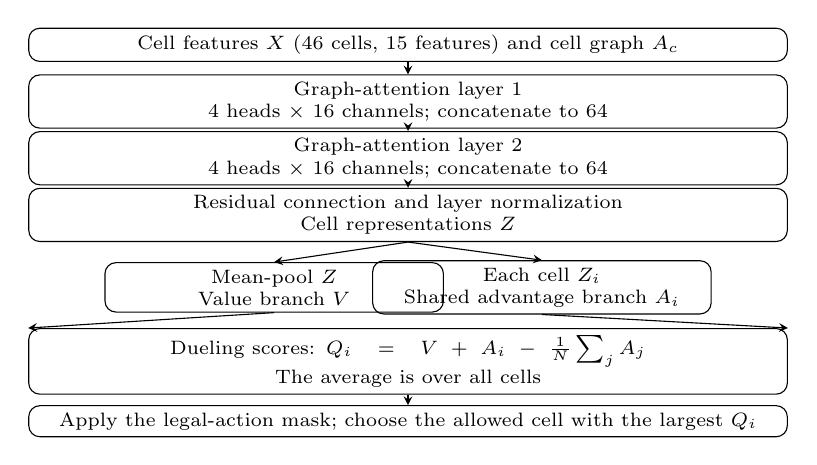
\begin{tikzpicture}[
  >=stealth,
  font=\scriptsize,
  block/.style={draw,rounded corners,align=center,text width=0.78\columnwidth,inner sep=2.5pt},
  branch/.style={draw,rounded corners,align=center,text width=0.34\columnwidth,inner sep=2.5pt}
]
  \node[block] (input) at (0,0) {Cell features $X$ (46 cells, 15 features) and cell graph $A_c$};
  \node[block] (gatone) at (0,-0.72) {Graph-attention layer 1\\4 heads $\times$ 16 channels; concatenate to 64};
  \node[block] (gattwo) at (0,-1.44) {Graph-attention layer 2\\4 heads $\times$ 16 channels; concatenate to 64};
  \node[block] (residual) at (0,-2.16) {Residual connection and layer normalization\\Cell representations $Z$};
  \node[branch] (value) at (-1.7,-3.08) {Mean-pool $Z$\\Value branch $V$};
  \node[branch] (advantage) at (1.7,-3.08) {Each cell $Z_i$\\Shared advantage branch $A_i$};
  \node[block] (combine) at (0,-4.02) {Dueling scores: $Q_i=V+A_i-\frac{1}{N}\sum_j A_j$\\The average is over all cells};
  \node[block] (mask) at (0,-4.78) {Apply the legal-action mask; choose the allowed cell with the largest $Q_i$};
  \draw[->] (input.south)--(gatone.north);
  \draw[->] (gatone.south)--(gattwo.north);
  \draw[->] (gattwo.south)--(residual.north);
  \draw[->] (residual.south)--(value.north);
  \draw[->] (residual.south)--(advantage.north);
  \draw[->] (value.south)--(combine.north west);
  \draw[->] (advantage.south)--(combine.north east);
  \draw[->] (combine.south)--(mask.north);
\end{tikzpicture}
  \caption{Graph-attention encoder and dueling action-value head. The cell graph guides information sharing. The legal-action mask is applied after the network calculates a score for each cell.}
  \label{fig:gat_dueling}
\end{figure}

\subsection{Training and frozen checkpoints}
Training follows a repeated loop: the policy observes the simulator, chooses an allowed cell, and receives the next observation and reward. The model then learns from stored transitions. During exploration, it uses $\epsilon$-greedy choice among allowed actions. It chooses randomly with probability $\epsilon$ and otherwise chooses the action with the highest Q-value. $\epsilon$ stays at 1 for the first 2,000 simulator steps, then decreases linearly to 0.05 over the next 100,000 steps. The replay buffer holds 20,000 transitions. Each transition stores the observation, allowed-action mask, chosen action, reward, terminal flag, and actual interval length. After the first 2,000 steps, the model samples 32 transitions and updates every four simulator steps. We use Adam with a 0.001 learning rate, Huber loss, and a maximum gradient norm of 10. The target network is copied from the online network every 1,000 optimizer updates. For each update, the online network chooses the next allowed action, and the target network gives its value:
\begin{equation}
 y_t=\begin{cases}
 r_t,&\text{terminal},\\
 r_t+0.99^{\Delta_t/\Delta_0}Q_{\theta^-}(o_{t+1},a_{t+1}^{\star}),&\text{otherwise}.
 \end{cases}
 \label{eq:target}
\end{equation}
Here, $a_{t+1}^{\star}=\arg\max_{i\in\mathcal{A}_{t+1}}Q_\theta(o_{t+1},i)$ is the allowed next action with the highest online-network score. For a terminal transition, the target is just the current reward; there is no future value. This is a Double-DQN update with a time-adjusted discount for a shortened final interval \cite{mnih2015,vanhasselt2016,velickovic2018,wang2016}.

We tested seven handover penalties: $c_H\in\{0.25,0.375,0.5,0.625,0.75,0.875,1.0\}$. Four candidates advanced to the medium training budget, and three continued to the full budget. We checked them on six fixed development routes. A candidate passed only if every tested seed had higher throughput than the configured A3-style controller and no more handovers, ping-pongs, or weak-service time. Among the candidates that passed, $c_H=0.875$ had the highest throughput.

With $c_H$ fixed at 0.875, we trained three policies using seeds 17, 27, and 37. Each followed the same plan of 300 journeys and completed 380,423 simulator steps. The journeys had 300 different route IDs, although some routes may share road segments. The evaluation uses these three trained policies.

We checked saved checkpoints on the same six development routes and kept one eligible checkpoint for each seed. The selected checkpoints are from steps 380,423, 280,778, and 380,423 for seeds 17, 27, and 37. Seed 27's later checkpoint failed the ping-pong check, so we kept its earlier checkpoint. These are three trained policies, not a large set of independent training runs. We did not use test results to choose checkpoints or seeds. Figure~\ref{fig:training} shows throughput and handover rate at the recorded checkpoints; it does not show episode reward or training loss.

\noindent\begin{minipage}{0.98\columnwidth}
\hrule\vspace{2pt}
\textbf{Algorithm 1. Training and checkpoint selection}\par
\textbf{Input:} simulator, fixed route plan, cell graph, $c_H=0.875$, and one training seed.\par
\textbf{Output:} one saved policy checkpoint.\par\vspace{-2pt}
\begin{enumerate}
  \setlength{\itemsep}{1pt}\setlength{\topsep}{2pt}\setlength{\parsep}{0pt}
  \item Initialize the online network, its target copy, and an empty replay buffer.
  \item For each of 300 journeys, observe the allowed actions. Choose one using the current $\epsilon$-greedy rule, run the simulator for the interval, and store the resulting transition, including its duration and action masks.
  \item Every four simulator steps after the first 2,000 steps, sample 32 transitions. Use Equation~\ref{eq:target} to form the targets, then update the online network with Huber loss and Adam. Limit the gradient norm to 10 and copy the online weights to the target network every 1,000 optimizer updates.
  \item Reduce $\epsilon$ from 1 to 0.05 over the next 100,000 steps. Continue until the 300 journeys are complete.
  \item Check saved checkpoints on the six development routes. Apply the development gate and freeze the selected checkpoint for evaluation.
\end{enumerate}
\vspace{-3pt}\hrule
\end{minipage}

\begin{figure}[H]\centering
  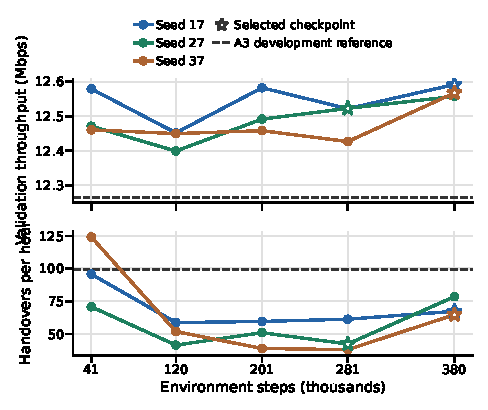
\includegraphics[width=0.98\linewidth]{Graphics/training_validation_progress.pdf}
  \caption{Development validation at five checkpoints from 41,125 to 380,423 environment steps, using the same six routes and conditions for each seed. Stars identify the frozen checkpoints selected by the full development gate; dashed lines show the A3 reference. Seed 27's 380,423-step checkpoint failed the ping-pong gate, so its 280,778-step checkpoint was retained. These fixed-route checkpoint measurements are not per-episode training returns.}
  \label{fig:training}
\end{figure}

\subsection{Trained-policy operation}
At each decision, the simulator provides the cell features and allowed-action mask. The graph encoder combines information from connected cells. The dueling head scores each cell, and the controller selects the allowed cell with the highest score. If this is a different cell, the simulator records a handover and pauses service for 0.1 s. It then advances the traffic and service models and returns the next observation and reward. During evaluation, the saved policy always chooses the allowed action with the highest score. It does not explore, save new transitions, or update its weights.

\subsection{Reproducibility and evaluation boundaries}
For repeatability, we keep the route splits, scenario seeds, feature definitions, radio settings, and selected checkpoints. Each controller uses the same route, layout, and condition group. We report the three learned seeds separately. The result files include throughput, handover rate, weak-service time, ping-pongs, completed short stays, and background service. Rates use the matching total simulation time. The uncertainty analysis keeps cases from the same routes together. These steps make the simulator tests easier to repeat, but they do not remove the study's limits. The model uses a fixed travel speed, simulator information and route look-ahead, simplified resource sharing, and assumed radio and load settings. Roads also overlap between training and reserved test routes. Pokhara tests use different roads and simulated cell layouts, so they are not field validation. The study does not show that training has converged, that graph attention caused the results, or that the controller is ready for commercial use.

\section{Evaluation Protocol}
\subsection{Reference controller and matched runs}
We compare three trained policies, with their weights fixed, against the configured A3-style controller. The reference uses 3 dB hysteresis and a 0.64 s time-to-trigger. The simulator checks the condition every 0.5 s. If the condition remains true, the handover starts 1.0 s after the first qualifying sample. This controller does not include every measurement filter, report delay, signal exchange, or reconnection step used in a live LTE network. We call it A3-style because it is a simulation reference, not a full LTE implementation.

For each case, all four controllers use the same route, radio and traffic seeds, journey length, and starting cell. The recorded simulator-state digests also match. The controllers can then make their own choices under the same starting conditions. The main test has 2,556 runs for 639 reserved cases and 2,160 runs for 540 transfer groups. We later added 639 original-area runs and 540 Pokhara runs for the load-aware comparison. We report each trained policy separately.

\subsection{Measures, diagnostic comparison, and uncertainty}
Our main measure is delivered throughput: total data received by the UE divided by the total simulation time. We also count handovers and ping-pongs, measure time below the $-120$ dBm RSRP threshold, and report how many completed cell stays after a handover last less than 5 s. We do not count the first stay or the final stay, because the final one ends when the route ends. We use these outcomes to describe service and switching. We do not use the training reward as an evaluation measure.

We kept the case-level records for all 639 reserved cases and 540 transfer groups. We calculated paired 95\% confidence intervals for throughput differences with 2,000 cluster-bootstrap samples. Each sample keeps results from the same group together so the controller comparisons remain paired. For the original area, the groups are the 102 origin--destination pairs, with both travel directions together. For Pokhara, the groups are the 60 routes, with each route's layouts and conditions kept together. These intervals describe the saved policies and scenarios tested here. They do not include changes from new training runs, other cities, or a wider range of cell layouts.

We added the load-aware rule after looking at the main A3-versus-learned results. We tried nine settings on six development routes: switching margins of 0.5, 1, or 2 Mbps and minimum stay times of 1, 3, or 5 s. A setting passed only if it gave higher throughput than A3 without more handovers, ping-pongs, or weak-service time. None passed. We kept the setting with the fewest failed checks for a diagnostic comparison only. It is named \texttt{load\_m2\_d5}; it uses a 2 Mbps margin and a 5 s minimum stay. If RSRP falls below $-120$ dBm, the rule can ignore both limits and switch to the strongest allowed neighbour. We fixed this setting before the additional 1,179 runs. No training or setting search was done during those runs. Because this rule was added after we saw the main results, it is not a planned baseline.

\section{Results}
\subsection{Reserved route cases}
Table~\ref{tab:heldout} shows the results for all 639 reserved cases. Figure~\ref{fig:paired} shows how throughput, handovers, and ping-pongs changed from A3 in each paired case. All three learned policies have 8.86--9.99\% higher aggregate throughput and 36.1--53.0\% fewer handovers per hour than A3. They also have fewer ping-pongs and less time below the weak-signal threshold. However, each has a higher share of completed stays shorter than 5 s.

The average paired throughput gains are $+1.147$ Mbps for seed 17 (95\% CI $[0.894,1.398]$), $+1.017$ Mbps for seed 27 ($[0.758,1.269]$), and $+1.032$ Mbps for seed 37 ($[0.791,1.271]$). Throughput is higher than A3 in 463, 415, and 418 of the 639 cases for these seeds. Other graph-based vehicle handover work also reports service and switching measures, though it uses different settings \cite{mehregan2025}.

\begin{table}[H]
  \caption{Aggregate outcomes for 639 reserved route cases. Weak service is the percentage of time with serving-cell RSRP below $-120$ dBm. Short stay is the percentage of completed handover-entered stays lasting less than 5 s; the initial stay and the final stay, which is cut short by the route ending, are excluded. Ping-pong values are counts. Load M2/D5 is the later-added load-aware diagnostic, which did not pass the development gate.}
  \label{tab:heldout}
  \centering\scriptsize\setlength{\tabcolsep}{2.4pt}
  \begin{tabular}{lrrrrr}
    \toprule
    Controller & Throughput & HO/h & Ping-pong & Weak-service & Short stay \\
    & (Mbps) & & (count) & (\%) & (<5 s, \%) \\
    \midrule
    A3-style & 11.477 & 109.60 & 652 & 12.10 & 26.49 \\
    Seed 17 & 12.624 & 69.68 & 147 & 5.93 & 37.62 \\
    Seed 27 & 12.494 & 51.51 & 17 & 6.20 & 30.27 \\
    Seed 37 & 12.509 & 70.05 & 37 & 6.24 & 43.73 \\
    Load M2/D5 & 12.072 & 298.62 & 2,582 & 5.86 & 21.08 \\
    \bottomrule
  \end{tabular}
\end{table}

\begin{figure*}[t]
  \centering
  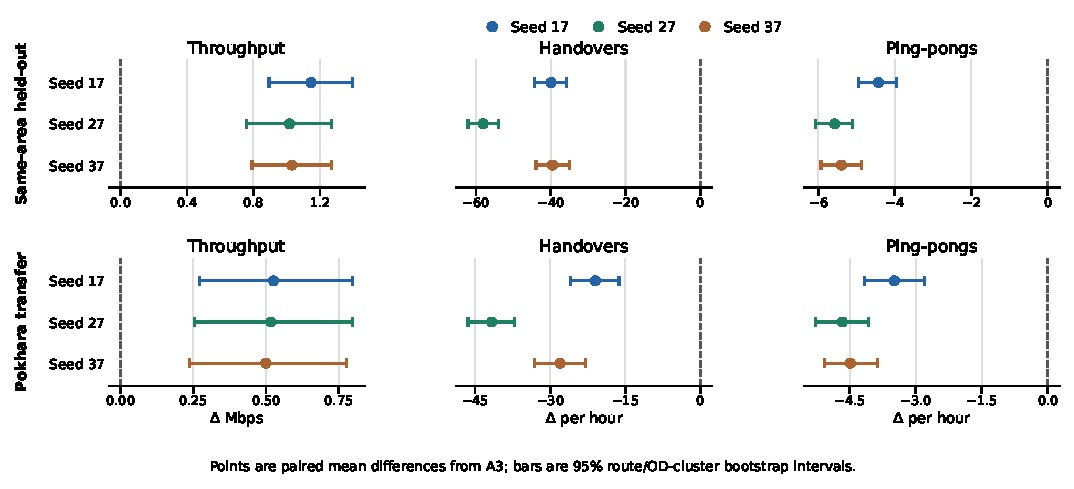
\includegraphics[width=\textwidth]{Graphics/paired_primary_outcomes.pdf}
  \caption{Paired differences from the configured A3-style reference on the 639 reserved routes and 540 Pokhara transfer groups. Negative handover and ping-pong differences indicate lower event rates. Error bars are 95\% cluster-bootstrap intervals (2,000 resamples; 102 OD-group clusters for reserved routes and 60 route clusters for transfer). All five outcomes, including weak-service time and short stays, are reported in Tables~\ref{tab:heldout} and~\ref{tab:pokhara}. These intervals are conditional on the three frozen policies and sampled scenarios.}
  \label{fig:paired}
\end{figure*}

The load-aware diagnostic has 0.595 Mbps higher aggregate throughput than A3 (95\% CI $[0.386,0.810]$), but it is higher in only 249 cases and lower in 390. It makes 189.02 more handovers per hour and has 1,930 more ping-pongs. It reduces weak-service time by 6.24 percentage points and short stays by 5.40 points.

Compared with Load M2/D5, the mean paired throughput gains are $+0.552$ Mbps for seed 17 (95\% CI $[0.441,0.659]$), $+0.422$ Mbps for seed 27 ($[0.310,0.535]$), and $+0.437$ Mbps for seed 37 ($[0.331,0.550]$). They also make fewer handovers and ping-pongs, but spend slightly more time in weak service and have more short stays. The diagnostic was added after the main results and did not pass the development check, so it is not a qualified baseline.

\subsection{Pokhara transfer evaluation}
The transfer test includes all 540 groups from 60 Pokhara routes, three simulated cell layouts, and three radio/traffic condition pairs. Table~\ref{tab:pokhara} shows that the learned policies have 3.66--3.85\% higher aggregate throughput than A3. They also make fewer handovers and ping-pongs and spend less time in weak service. Short-stay results differ by policy: seed 27 is lower than A3, while seeds 17 and 37 are higher.

The average paired throughput gains over A3 are $+0.526$ Mbps for seed 17 (95\% CI $[0.272,0.799]$), $+0.517$ Mbps for seed 27 ($[0.254,0.797]$), and $+0.499$ Mbps for seed 37 ($[0.237,0.777]$). Throughput is higher in 349, 351, and 315 groups, with 4, 6, and 5 ties. Other graph-reinforcement-learning work has tested changes in network layouts, but it studies a different task \cite{salvatori2026}.

\begin{table}[H]
  \caption{Aggregate outcomes for all 540 Pokhara transfer groups. Weak service is the percentage of time with serving-cell RSRP below $-120$ dBm. Short stay is the percentage of completed handover-entered stays lasting less than 5 s; the initial stay and the final stay, which is cut short by the route ending, are excluded. Ping-pong values are counts. The cell layouts are synthetic, and Load M2/D5 is the later-added diagnostic.}
  \label{tab:pokhara}
  \centering\scriptsize\setlength{\tabcolsep}{2.4pt}
  \begin{tabular}{lrrrrr}
    \toprule
    Controller & Throughput & HO/h & Ping-pong & Weak-service & Short stay \\
    & (Mbps) & & (count) & (\%) & (<5 s, \%) \\
    \midrule
    A3-style & 13.652 & 88.52 & 336 & 4.42 & 25.55 \\
    Seed 17 & 14.178 & 67.56 & 92 & 1.32 & 36.00 \\
    Seed 27 & 14.169 & 46.83 & 9 & 1.45 & 22.72 \\
    Seed 37 & 14.151 & 60.52 & 22 & 1.39 & 33.53 \\
    Load M2/D5 & 13.969 & 234.62 & 341 & 0.67 & 6.40 \\
    \bottomrule
  \end{tabular}
\end{table}

Load M2/D5 has 0.317 Mbps higher aggregate throughput than A3 (95\% CI $[0.003,0.664]$). It is higher in 145 groups, lower in 393, and tied in 2. Compared with Load M2/D5, the mean paired throughput gains are $+0.209$ Mbps for seed 17 (95\% CI $[0.073,0.310]$), $+0.200$ Mbps for seed 27 ($[0.077,0.297]$), and $+0.183$ Mbps for seed 37 ($[0.044,0.286]$). They make fewer handovers and ping-pongs than the diagnostic, but spend more time in weak service and have more short stays. Using the rounded table values, these increases are about 0.65--0.78 percentage points for weak service and 16.32--29.60 points for short stays. These intervals describe the fixed policies and tested cases. They do not cover new training runs, cities, or cell layouts.

\section{Discussion and Limitations}
In the reserved and Pokhara tests, all three learned policies have higher aggregate throughput and fewer handovers, ping-pongs, and weak-service time than the A3-style controller. Short stays increase for all three policies on the reserved routes and for two policies in the Pokhara tests. This shows that throughput and handover count do not tell the whole story. Compared with the load-aware diagnostic, the learned policies make fewer handovers, but some of them have more weak-service time or short stays. No one controller is better on every measure.

We added the load-aware comparison after seeing the main results. All nine settings failed the development check. We froze the setting with the fewest failed checks before running the extra reserved and Pokhara cases. This is still a later-added comparison, not a baseline chosen before the main study. A future study should tune a load-aware controller using the same development rules and choose it before testing the reserved routes.

The results also have other limits. The radio, traffic, and resource-sharing models are simplified. The controller uses simulator estimates for possible cells and information about the next point on the route. The A3-style reference is also a simplified version of the standard procedure. Although the reserved routes were not used for training, 67.1\% of their distinct directed road edges also appeared in the 300 training journeys. The Pokhara tests use real road shapes but simulated cell layouts and one city area, so they are not field tests or evidence for other cities. We trained only three policies, and the confidence intervals do not include variation from more training runs or real networks. We also did not compare against a DDQN without graph attention, so we cannot say that graph attention caused the observed gains. These results do not show that the controller is ready for commercial use.

\section{Conclusion}
We tested three fixed learned policies on 639 reserved route cases and 540 Pokhara transfer groups. All three had higher aggregate throughput and fewer handovers than the A3-style controller. They also had fewer ping-pongs and less weak-service time. Short stays increased for every policy on the reserved routes and for two policies in the transfer tests. The load-aware diagnostic did not pass the development check, and it had many handovers and ping-pongs. These findings apply to the simulations used here. They do not show what would happen in other cities, with new training runs, or in a live network. Shared roads, simulated Pokhara cell layouts, simulator-only information, and the lack of a graph-attention ablation limit the conclusions. More simulation and a comparison without graph attention are needed before field tests.

\phantomsection
\section*{Data and Code Availability}
The research code and manuscript files are available at \url{https://github.com/Sange-creator/toponet-research}. The route and cell-layout inputs, trained policy checkpoints, and complete case-level results are not included in the repository. The reported experiments therefore cannot be reproduced from the public repository alone.

\phantomsection
\bibliographystyle{unsrt}
\bibliography{refs}

\end{document}
